%!TEX root = ../../architekturdokumentation.tex
\chapter{Logische Architektur}

\section{3-Tier-Architektur}
	Um eine möglichst hohe Abstraktion unseres Codes zu erhalten, haben wir uns für eine 3-Tier-Architektur entschieden, die unsere Applikation in die drei Schichten Web, Service und DataAccesLayer (Dal) unterteilt. Alle Datenbankspezifischen Operationen sollen im DAL vorgenommen werden. Alle Zugriffe aus dem Web sollen über die Web-Layer behandelt werden. Die Zugriffe auf externe Schnittstellen über den Service-Layer.
	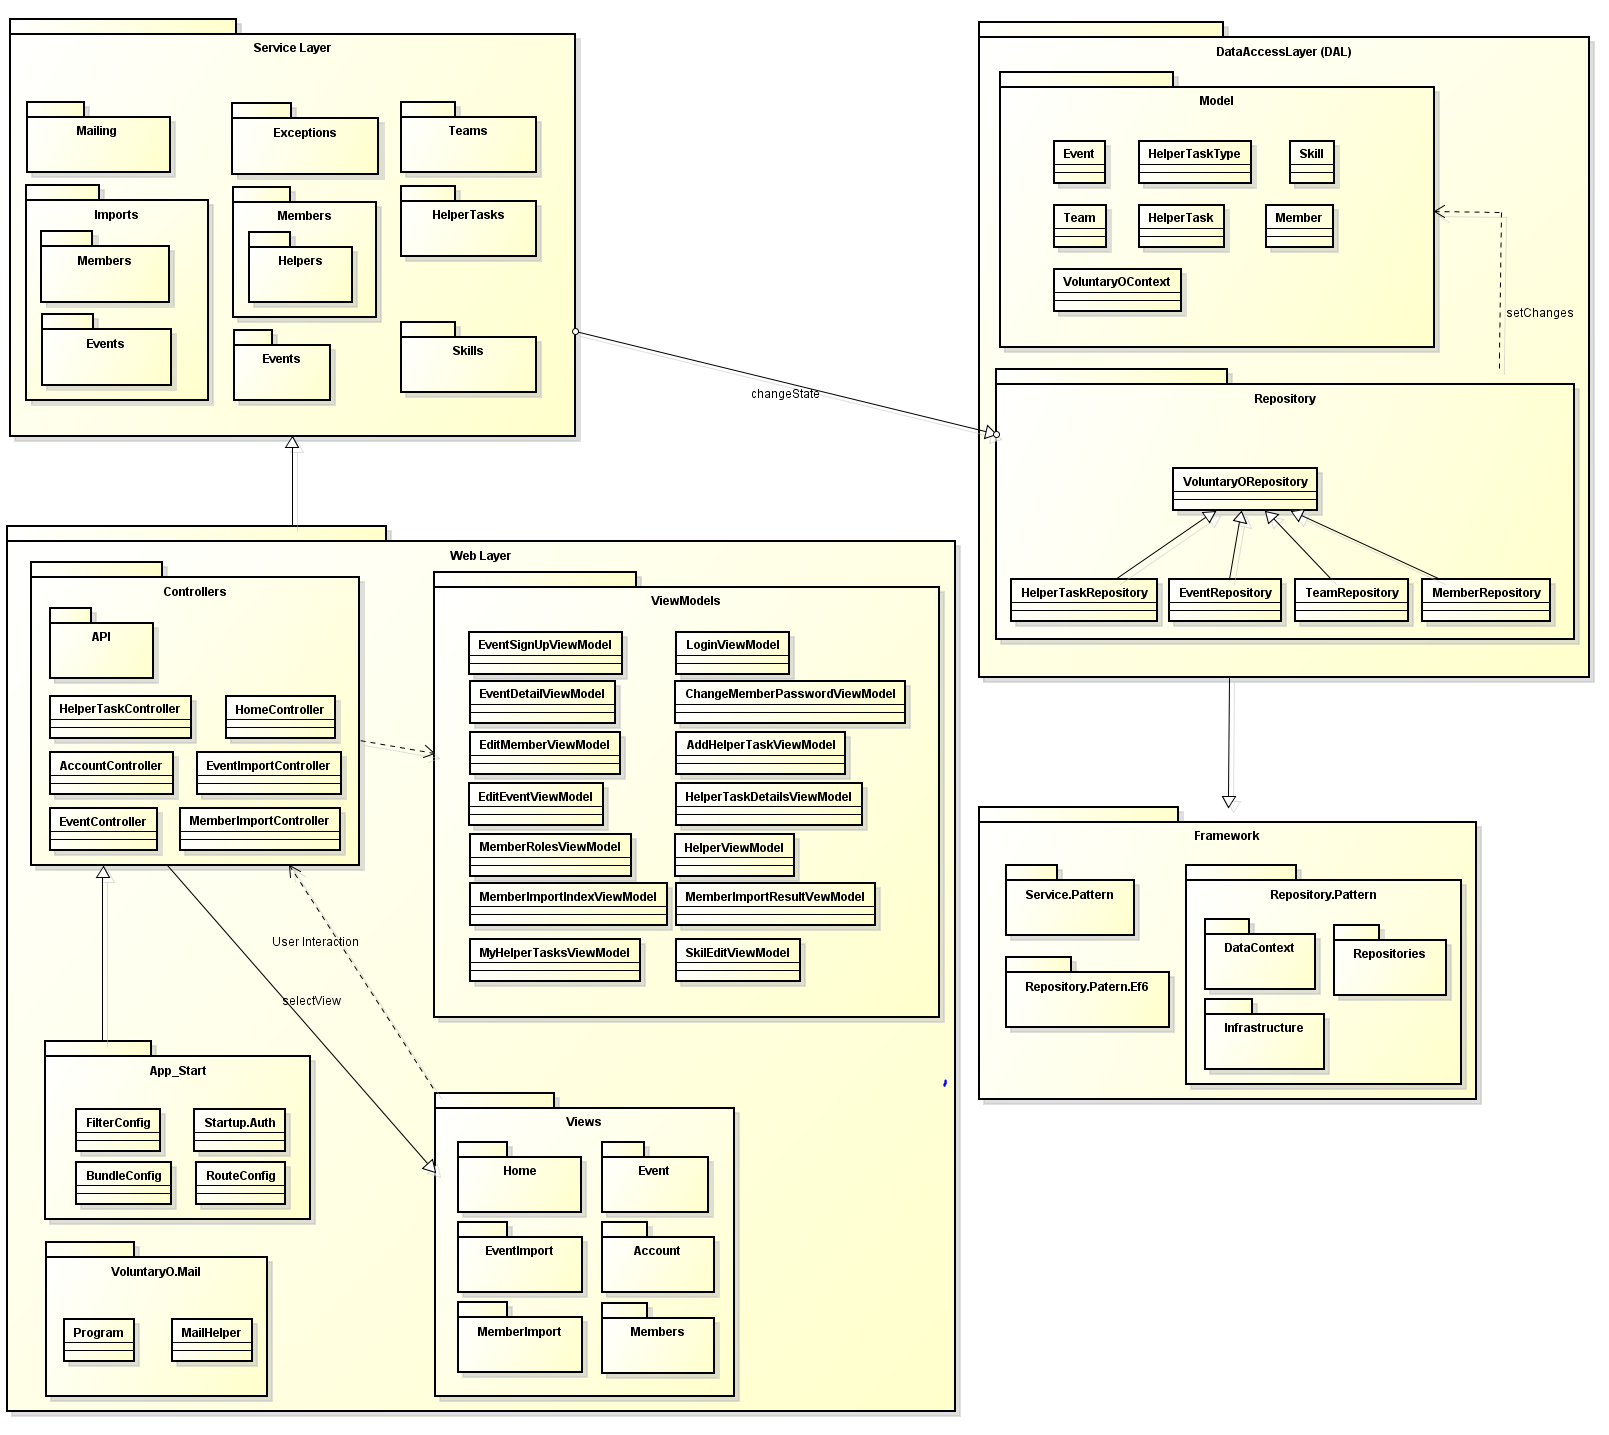
\includegraphics[width=\textwidth]{content/architekturdokumentation/images/LogischeArchitektur.png}

\section{VoluntaryO.Dal (Data Access Layer)}
    \begin{figure}[h]
  		\vspace{-5pt}
    	\centering
    	% VOLO-124
		% \includegraphics[width=\textwidth]{content/architekturdokumentation/images/domain.png}
  		\vspace{-25pt}
    	\caption{Domain in Subsystem VoluntaryO.Dal}
	\end{figure}

	\subsection{Mapping}
	Das Mapping wird mit dem \textit{modelBuilder} des Entity Framework (EF) gesteuert. Bspw.
	\begin{lstlisting}[language=CSharp, caption=Mapping in VoluntaryoContext.cs, label=lst:mappingcontextcs, firstnumber=1]
// TeamEventMapping
modelBuilder.Entity<Team>()
    .HasMany(t => t.Events)
    .WithMany(e => e.Teams)
    .Map(mc =>
    {
        mc.MapLeftKey("TeamID");
        mc.MapRightKey("EventID");
        mc.ToTable("TeamEventMappings");
    });
    \end{lstlisting}

	\subsection{Vergleich für Objekte}
	Einzig für die Member-Klasse wurde die Vergleichsmethode (Equals) überschrieben. Folgende Attribute der Klasse sind relevant:
	\\\begin{itemize}
		\item \textit{UserName}
		\item \textit{Firstname}
		\item \textit{Lastname}
		\item \textit{Birthdate}
	\end{itemize}

	\subsection{Repository / Unit of Work Pattern}
	Dieses Kapitel kann evtl. auch unter Service beschrieben werden.

\section{VoluntaryO.Service}

\section{VoluntaryO.Web}
